\section{Anden iteration}

\subsection{Integrationstest - Constant-load}

\subsubsection{Udgang}
\noindent Figur~\ref{fig: Out26V} viser det realiserede spændingsoutput ved 26V. Kanal et viser spændingsoutputtet, mens kanal to viser gate spændingen for MOSFET'en. Kanal to er brugt til at trigge på, ved alle constant-load målingerne. 
\begin{figure}[H]
	\center
	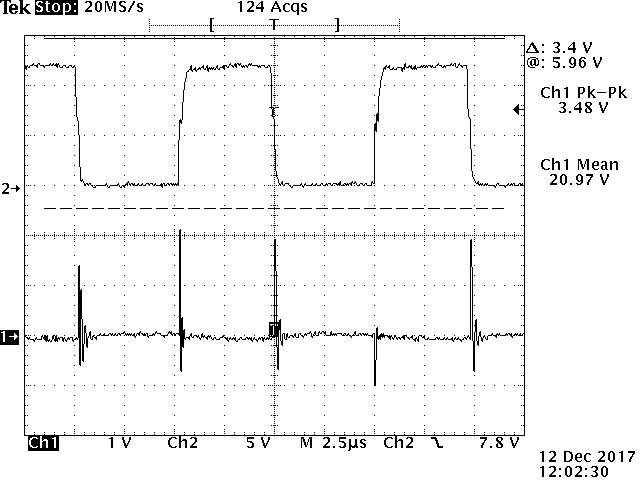
\includegraphics[max width=0.7\linewidth]{../dokumentation/tex/2iteration/billeder/Realisering/udgang_f_filter_2iteration.png}
	\caption{Spændingsoutput ved 26V}
	\label{fig: Out26V}
\end{figure}
\noindent Spændingen aflæses til at ligge på 20.97V. Yderligere observeres det, at der er swithing-spikes på omkring 3.48V pk-pk.

\subsubsection{MOSFET og diode}
\noindent Figur~\ref{fig: privolt} viser drain spændingen for MOSFET'en på kanal et, som også svarer til spændingen over den primære vikling i transformatoren.
\begin{figure}[H]
	\center
	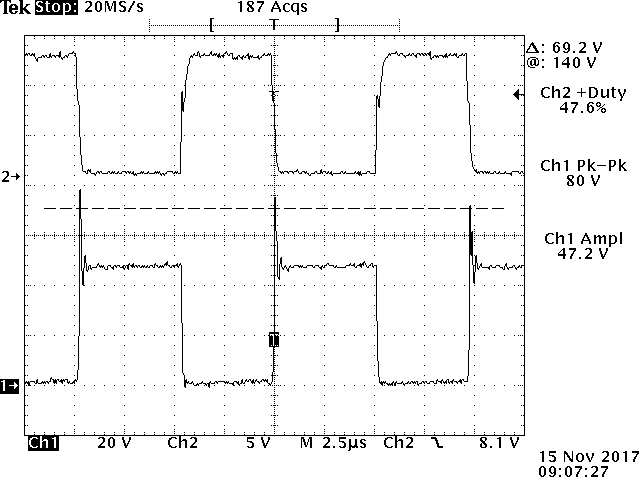
\includegraphics[max width=0.7\linewidth]{../dokumentation/tex/2iteration/billeder/Realisering/Transformator_Primar.png}
	\caption{Primær spænding}
	\label{fig: privolt}
\end{figure}
\noindent Spændingen over den primære vikling aflæses til en peak på 80V. Derudover aflæses den stationære spænding til, at ligge på 47V. 
På figur~\ref{fig: prizoom} er der zoomet ind på svingningerne omkring peakspændingen, som observeres ovenfor.
\begin{figure}[H]
	\center
	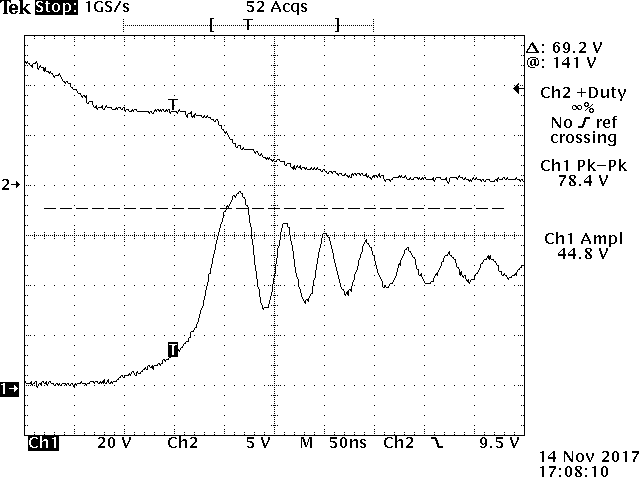
\includegraphics[max width=0.7\linewidth]{../dokumentation/tex/2iteration/billeder/Realisering/Transformator_Primarzoom.png}
	\caption{Zoomet på primær peak}
	\label{fig: prizoom}
\end{figure}
\noindent Svingningen for en periode aflæses til 40ns. Det svarer til en frekvens på $25MHz$. Samme fremgangsmetode er benyttet ved dioden, og målingerne herfra kan ses i dokumentationen, afsnit 5.9.1.

\noindent I tabel~\ref{tab:MOSDIODE} ses sammenhængen mellem simulering og realisering for dioden og MOSFET'en.
\begin{table}[H] 			
	\centering
	\begin{tabularx}{\textwidth}{|X|l|l|l|l|}
		\hline
		& \multicolumn{2}{|X|}{\textbf{Simulering}} & \multicolumn{2}{|X|}{\textbf{Realisering}} \\ \hline
		& MOSFET & Diode & MOSFET & Diode \\ \hline
		Stationær spænding & $48V$ & $46V$ & $47V$ & $45V$ \\ \hline
		Peakspænding & $93V$ & $80V$ & $80V$ & $60V$ \\ \hline
		Svingningsfrekvens & $29.41M\hertz$ & $33.33M\hertz$ & $25.00M\hertz$ & $28.57M\hertz$ \\ \hline
	\end{tabularx}
	\caption{Simulering og realisering af spændinger over MOSFET og diode}
	\label{tab:MOSDIODE}
\end{table}

\clearpage

\subsection{Integrationstest - Gain-fase måling}
Figur~\ref{fig:realisering_gain_fase_tot} viser et bode plot af den realiserede gain-fase for hele systemet sammen med det analyserede.
\begin{figure}[H]
	\center
	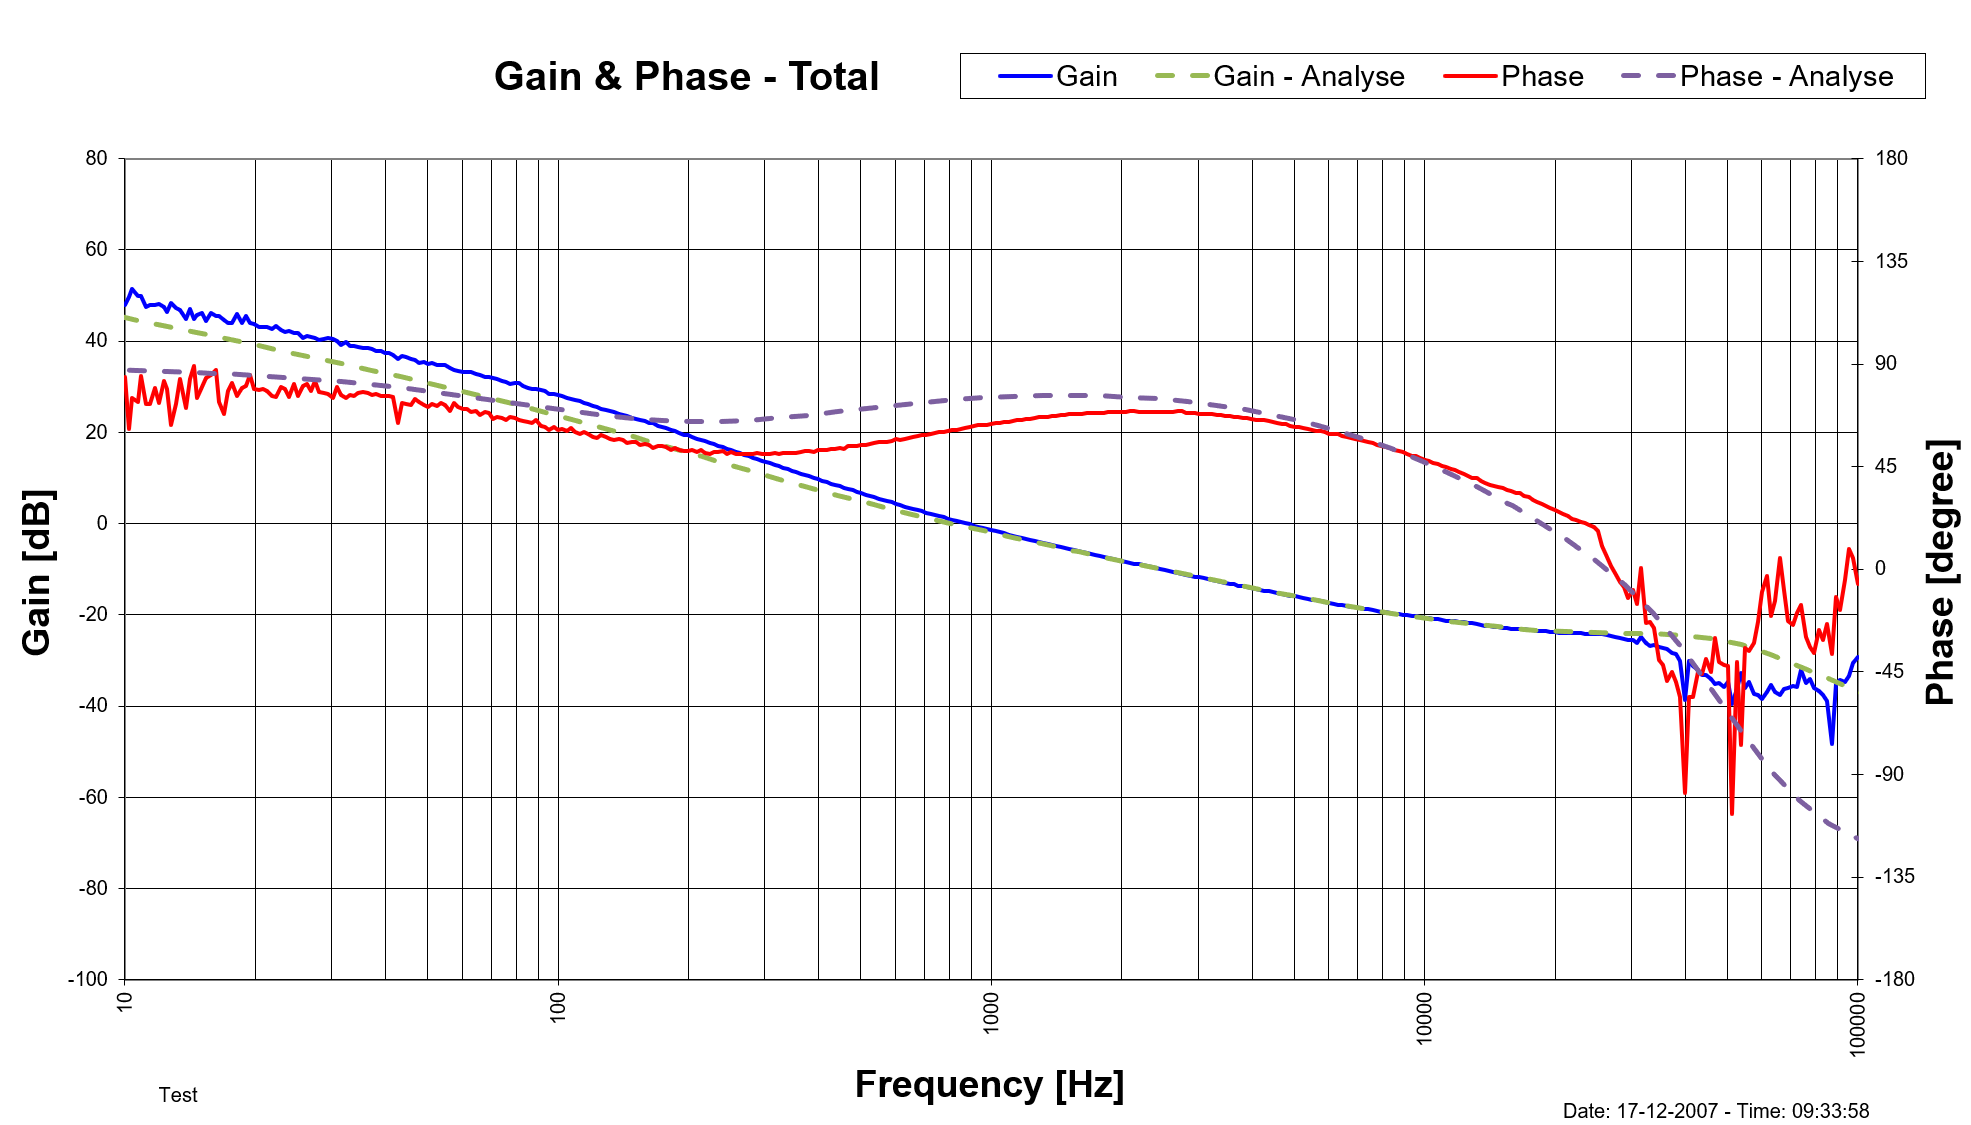
\includegraphics[max width=0.7\linewidth]{../dokumentation/tex/2iteration/billeder/Realisering/Realisering_gain_fase_tot.png}
	\caption{Realiseret og analytisk gain-fase for hele systemet}
	\label{fig:realisering_gain_fase_tot}
\end{figure}
\noindent Den blå linje er fasen for det realiserede, mens gain er den røde linje. Den grønne stiplede linje stammer fra den analyserede fase og den lila stiplede er det analyserede gain. Båndbredden for både analyse og fase aflæses til ca. $900Hz$. For det realiserede aflæses fase-marginen til ca. $62^\circ$ og gain-marginen til ca. $24dB$. Den analyserede fase-margin kan aflæses til $74.3^\circ$ med samme gain-margin, som det realiserede.

\subsection{Load-step}
Figur~\ref{fig:belastningsamlet} viser det realiserede load-step.
\begin{figure}[H]
	\center
	\includegraphics[max width=0.7\linewidth]{../dokumentation/tex/2iteration/billeder/Realisering/belastningsamlet.png}
	\caption{Realisering af load-step}
	\label{fig:belastningsamlet}
\end{figure}
\noindent Det aflæses at spændingen falder med ca. 700mV ved overgangen til $10\ohm$. Det tager ca. $1.5ms$ at regulere ind til den stationære værdi. Ved overgangen tilbage til $20\ohm$ stiger spændingen ca. $600mV$, og bruger igen $1.5ms$ på at regulere ind.